\section{Clustering}
	
		
		A series of different clustering algorithms are used:
		\begin{itemize}
			\item K-Means
			\item DBSCAN
			\item HDBSCAN
			\item Agglomerative clustering
		\end{itemize}
		
		The clusters obtained will be compared the original clusters using NMI
		
	\subsection{Zernike coefficients clustering}
		
		\subsubsection{K-Means}
			
			As K-Means allows for the number of clusters to define, and we know that there are 4 in the original dataset, K-Means is used to find 4 clusters.
			
			\begin{table}[h!]
				\centering
				\begin{tabular}{|c|c|}
					\hline
					\textbf{Number of clusters} & \textbf{Number of initializations}\\
					\hline
					4 & 10\\
					\hline
				\end{tabular}
				\caption{K-Means hyperparameter configuration for Zernike coefficients clustering}
			\end{table}
		
			The results are the following:
			
			\begin{figure*}[ht!]
				\centering
				\subfloat[Original cluster densities]{%
					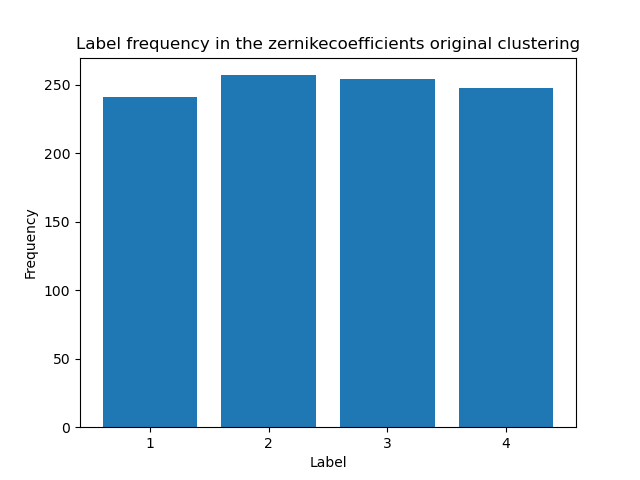
\includegraphics[width=0.45\textwidth]{mdid-zernikecoefficientsoriginaldensity.png}}
				\hspace{\fill}
				\subfloat[K-Means clusters densities]{%
					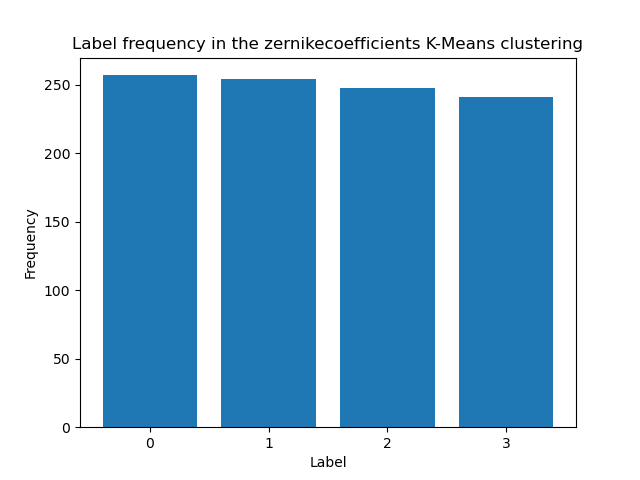
\includegraphics[width=0.45\textwidth]{mdid-zernikecoefficientsK-Meansdensity.png}}\\
				\subfloat[Original clusters]{%
					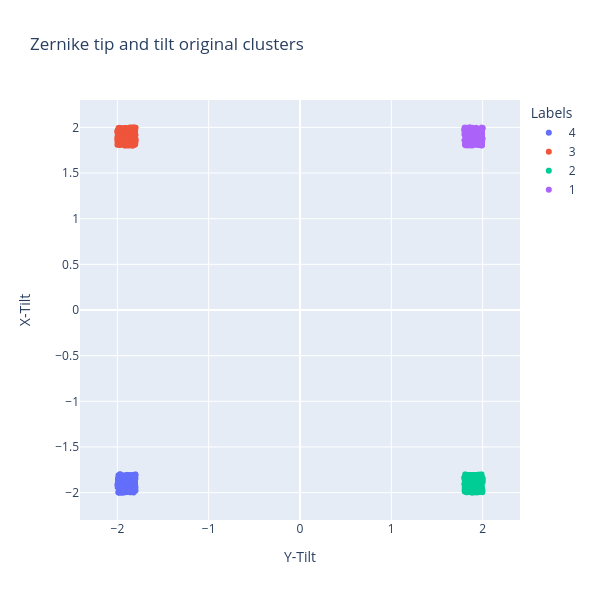
\includegraphics[width=0.45\textwidth]{mdid-zernikecoefficientsoriginalclusters.png}}
				\hspace{\fill}
				\subfloat[K-Means clusters]{%
					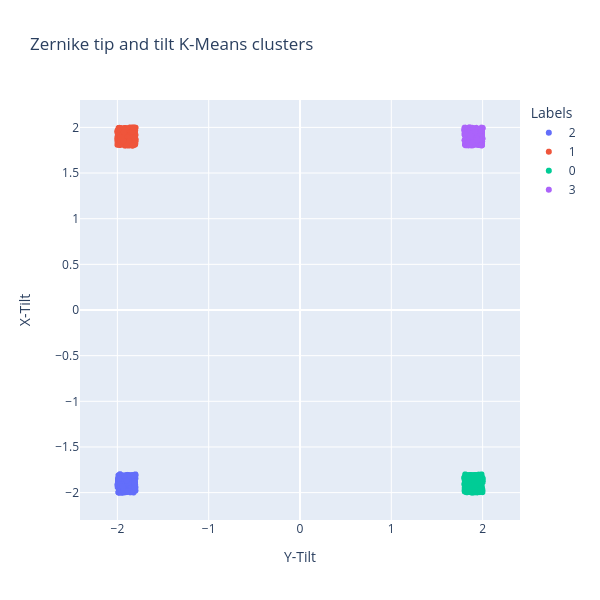
\includegraphics[width=0.45\textwidth]{mdid-zernikecoefficientsK-Meansclusters.png}}\\
					
				\subfloat[Original cluster samples]{%
					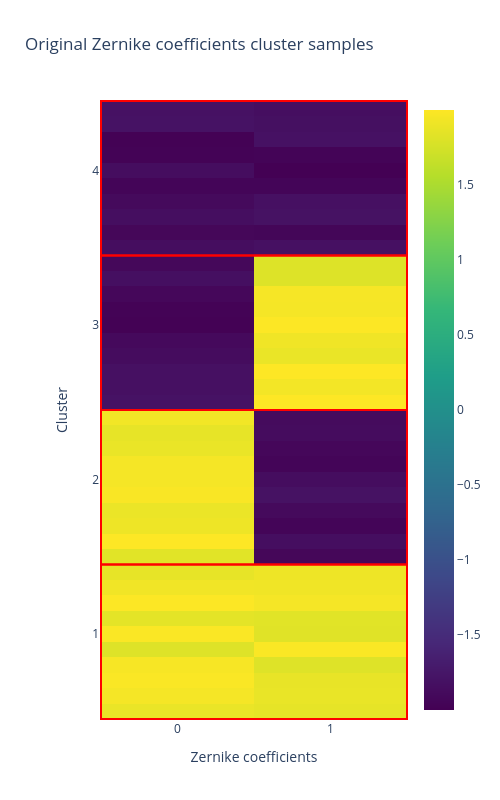
\includegraphics[width=0.4\textwidth]{mdid-zernikecoefficientsoriginalgridclusters.png}}
				\hspace{\fill}
				\subfloat[K-Means cluster samples]{%
					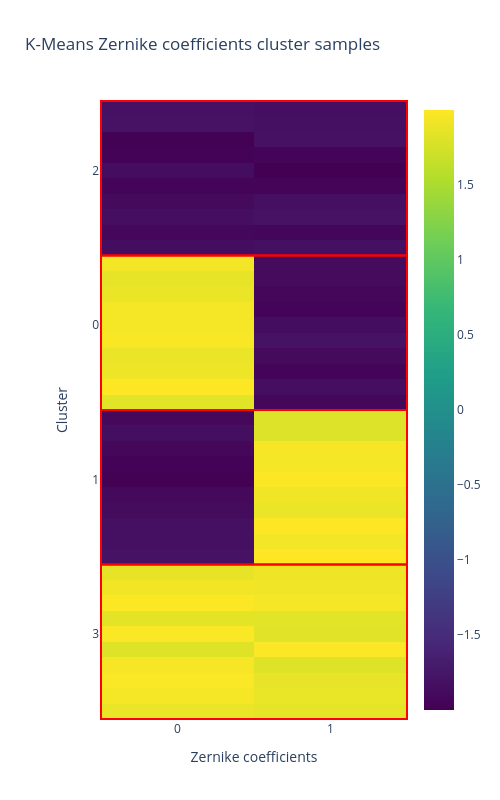
\includegraphics[width=0.4\textwidth]{mdid-zernikecoefficientsK-Meansgridclusters.png}}
				\caption{Comparison between original clustering and K-Means clustering}
			\end{figure*}
		\FloatBarrier
		
		\subsubsection{DBSCAN}
			
			A configuration that outputs 4 clusters is searched
			
			\begin{table}[h!]
				\centering
				\begin{tabular}{|c|c|}
					\hline
					\textbf{Number of neighbours} & \textbf{Epsilon}\\
					\hline
					5 & 0.3\\
					\hline
				\end{tabular}
				\caption{DBSCAN hyperparameter configuration for Zernike coefficients clustering}
			\end{table}
		
			The results are the following:
			
			\begin{figure*}[ht!]
				\centering
				\subfloat[Original cluster densities]{%
					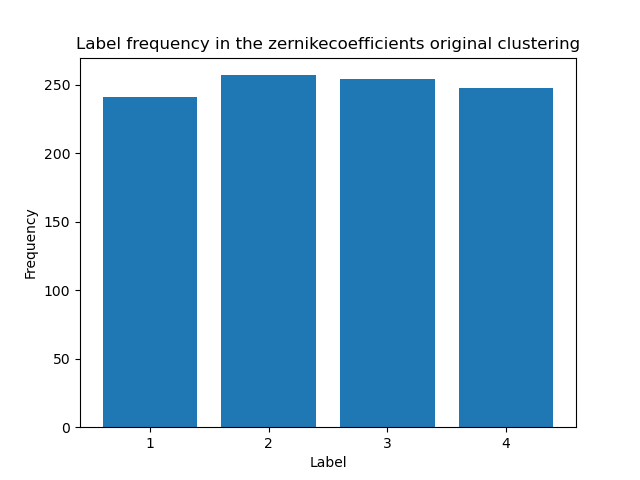
\includegraphics[width=0.45\textwidth]{mdid-zernikecoefficientsoriginaldensity.png}}
				\hspace{\fill}
				\subfloat[DBSCAN clusters densities]{%
					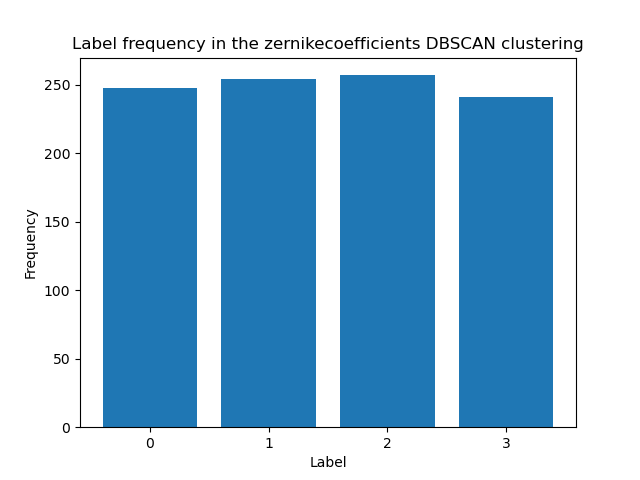
\includegraphics[width=0.45\textwidth]{mdid-zernikecoefficientsDBSCANdensity.png}}
				\\
				\subfloat[Original clusters]{%
					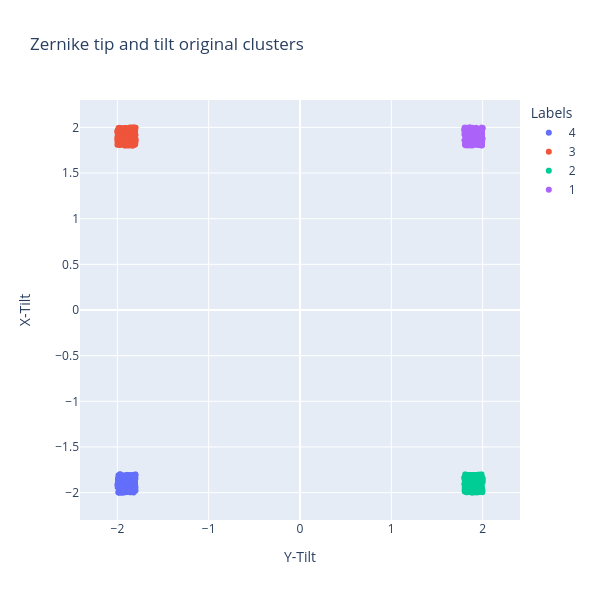
\includegraphics[width=0.45\textwidth]{mdid-zernikecoefficientsoriginalclusters.png}}
				\hspace{\fill}
				\subfloat[DBSCAN clusters]{%
					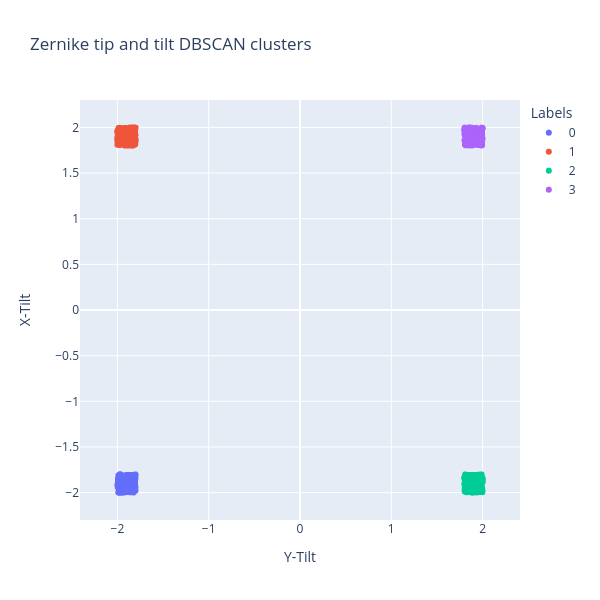
\includegraphics[width=0.45\textwidth]{mdid-zernikecoefficientsDBSCANclusters.png}}\\
					
				\subfloat[Original cluster samples]{%
					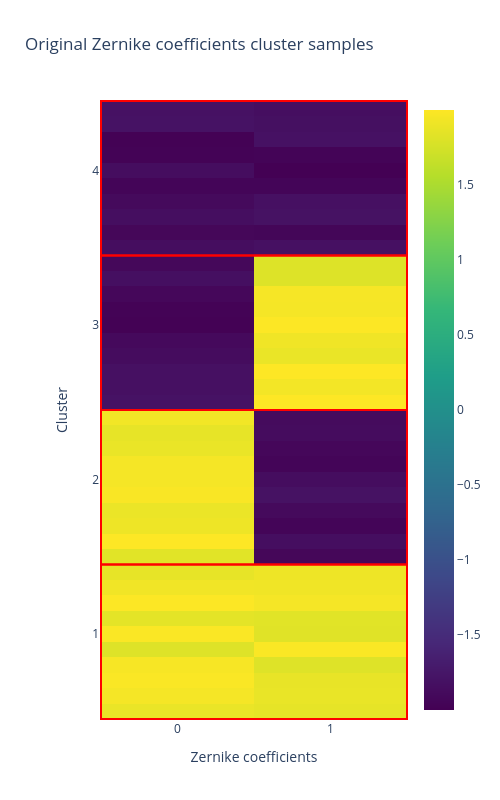
\includegraphics[width=0.4\textwidth]{mdid-zernikecoefficientsoriginalgridclusters.png}}
				\hspace{\fill}
				\subfloat[DBSCAN cluster samples]{%
					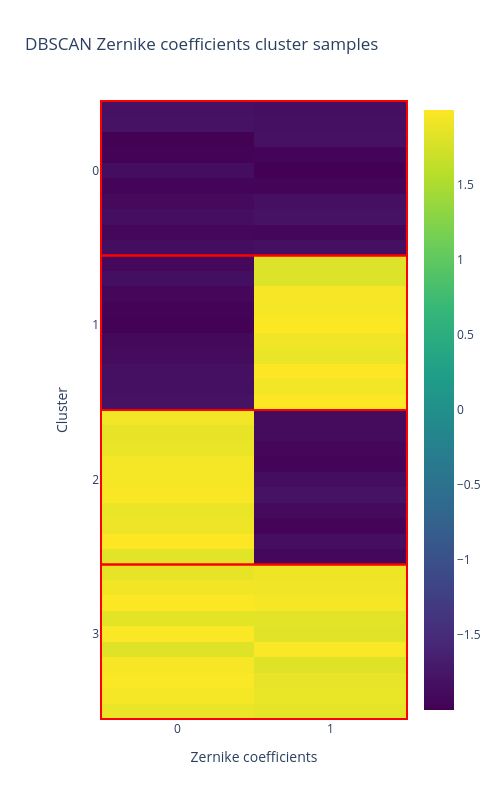
\includegraphics[width=0.4\textwidth]{mdid-zernikecoefficientsDBSCANgridclusters.png}}
				\caption{Comparison between original clustering and DBSCAN clustering}
			\end{figure*}
		\FloatBarrier
		
		\subsubsection{HDBSCAN}
			
			A configuration that outputs 4 clusters is searched.
			
			\begin{table}[h!]
				\centering
				\begin{tabular}{|c|c|}
					\hline
					\textbf{Minimum cluster size} \\
					\hline
					5 \\
					\hline
				\end{tabular}
				\caption{HDBSCAN hyperparameter configuration for Zernike coefficients clustering}
			\end{table}
			\FloatBarrier
			The results are the following:
			
			\begin{figure*}[ht!]
				\centering
				\subfloat[Original cluster densities]{%
					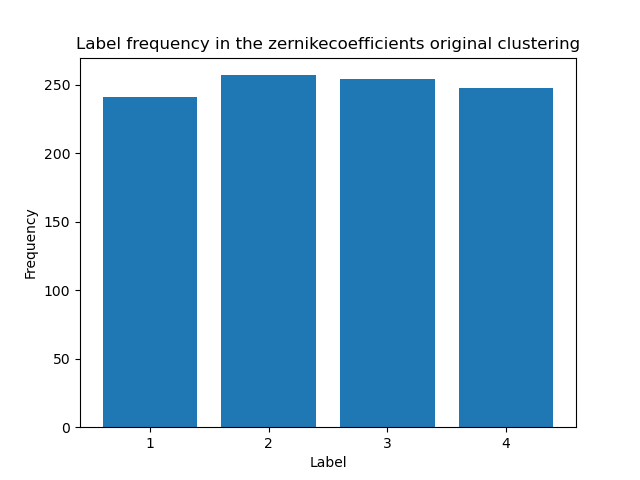
\includegraphics[width=0.45\textwidth]{mdid-zernikecoefficientsoriginaldensity.png}}
				\hspace{\fill}
				\subfloat[HDBSCAN clusters densities]{%
					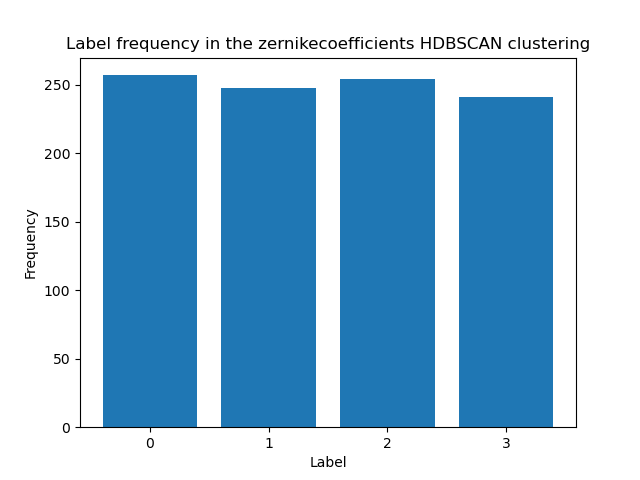
\includegraphics[width=0.45\textwidth]{mdid-zernikecoefficientsHDBSCANdensity.png}}
				\\
				\subfloat[Original clusters]{%
					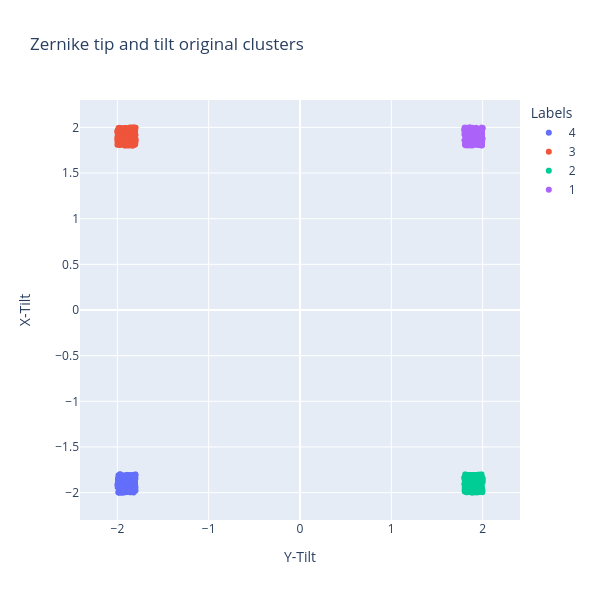
\includegraphics[width=0.45\textwidth]{mdid-zernikecoefficientsoriginalclusters.png}}
				\hspace{\fill}
				\subfloat[HDBSCAN clusters]{%
					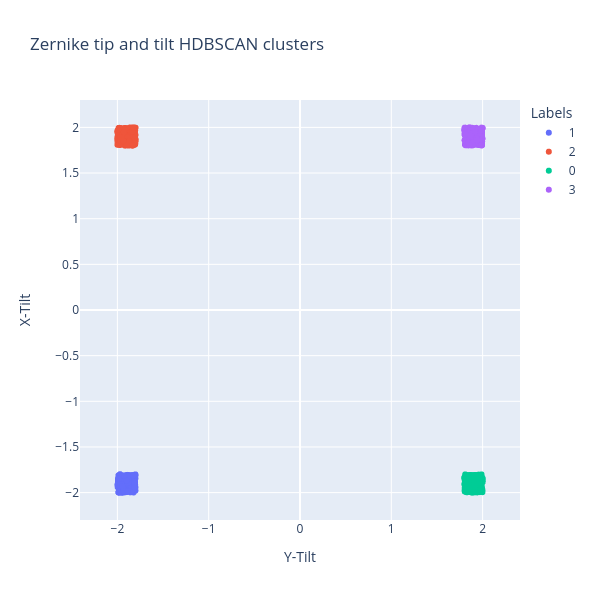
\includegraphics[width=0.45\textwidth]{mdid-zernikecoefficientsHDBSCANclusters.png}}\\
					
				\subfloat[Original cluster samples]{%
					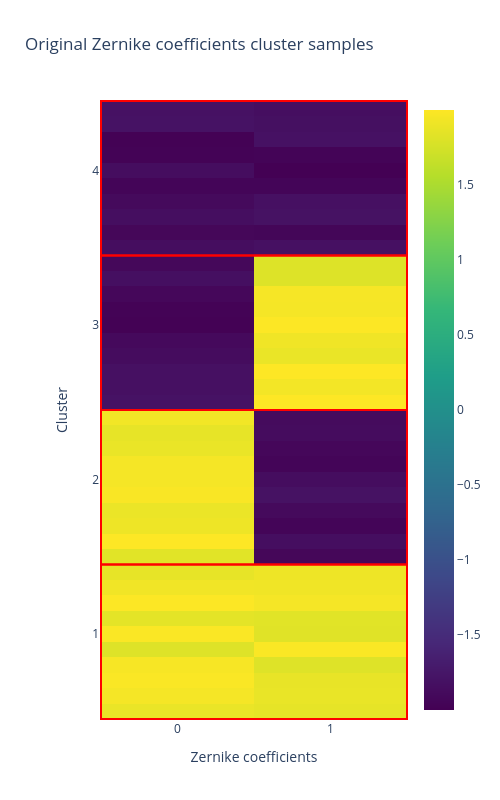
\includegraphics[width=0.4\textwidth]{mdid-zernikecoefficientsoriginalgridclusters.png}}
				\hspace{\fill}
				\subfloat[HDBSCAN cluster samples]{%
					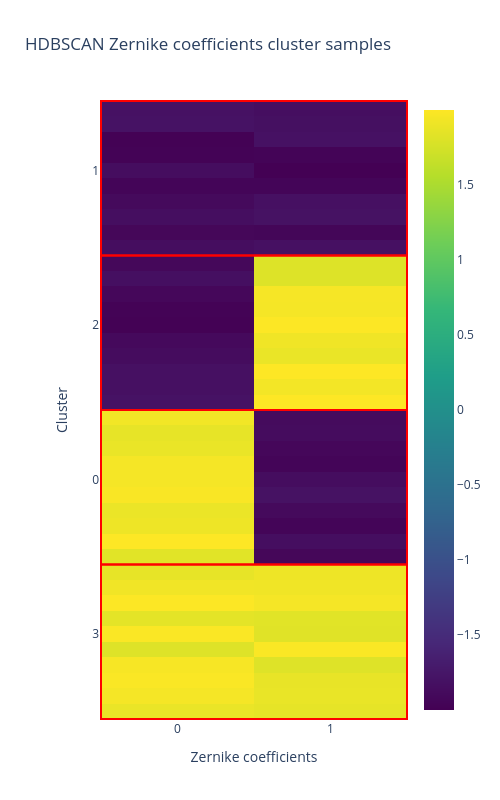
\includegraphics[width=0.4\textwidth]{mdid-zernikecoefficientsHDBSCANgridclusters.png}}
				\caption{Comparison between original clustering and HDBSCAN clustering}
			\end{figure*}
		\FloatBarrier
		
		\subsubsection{Agglomerative clustering}
			\begin{table}[h!]
				\centering
				\begin{tabular}{|c|c|}
					\hline
					\textbf{Number of clusters 4} \\
					\hline
					5 \\
					\hline
				\end{tabular}
				\caption{Agglomerative hyperparameter configuration for Zernike coefficients clustering}
			\end{table}
			\FloatBarrier
			The results are the following:
			
			\begin{figure*}[ht!]
				\centering
				\subfloat[Original cluster densities]{%
					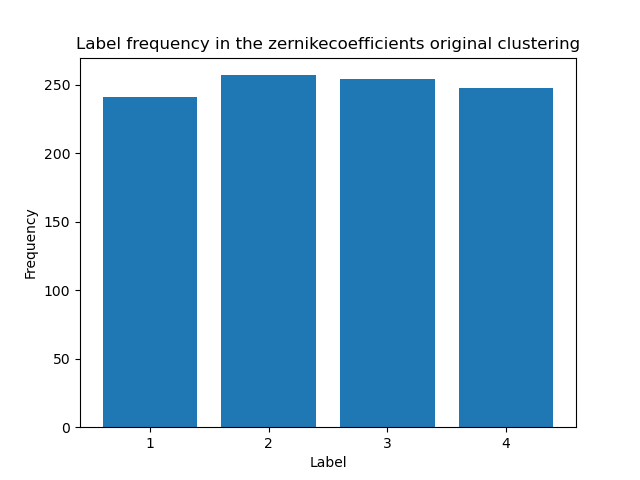
\includegraphics[width=0.45\textwidth]{mdid-zernikecoefficientsoriginaldensity.png}}
				\hspace{\fill}
				\subfloat[Agglomerative clusters densities]{%
					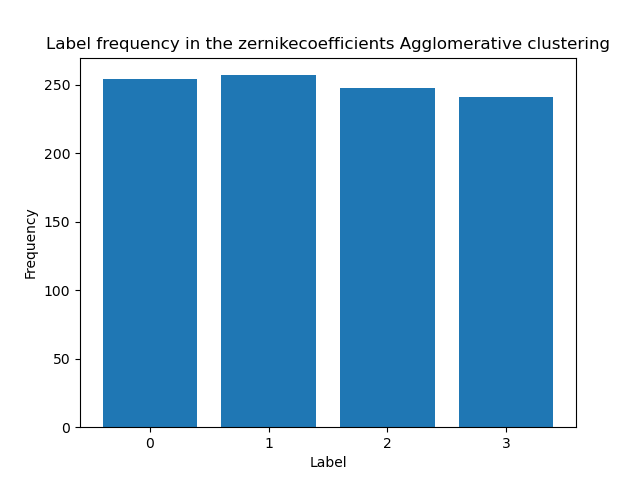
\includegraphics[width=0.45\textwidth]{mdid-zernikecoefficientsAgglomerativedensity.png}}
				\\
				\subfloat[Original clusters]{%
					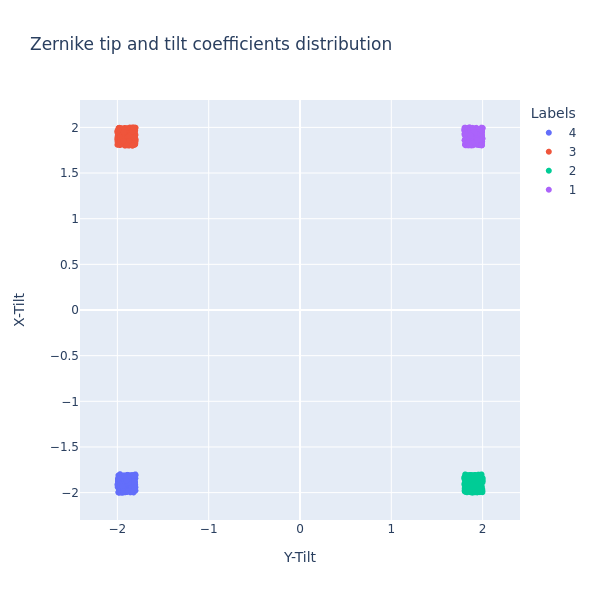
\includegraphics[width=0.45\textwidth]{mdid-originalclusters.png}}
				\hspace{\fill}
				\subfloat[Agglomerative clusters]{%
					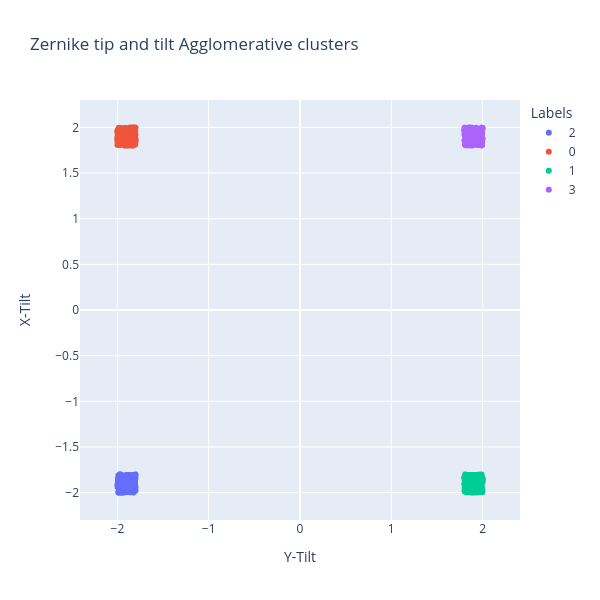
\includegraphics[width=0.45\textwidth]{mdid-zernikecoefficientsAgglomerativeclusters.png}}\\
					
				\subfloat[Original cluster samples]{%
					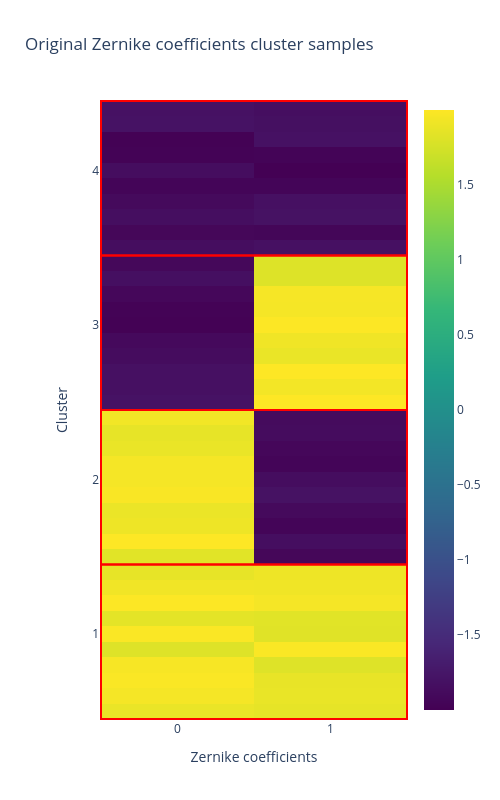
\includegraphics[width=0.4\textwidth]{mdid-zernikecoefficientsoriginalgridclusters.png}}
				\hspace{\fill}
				\subfloat[Agglomerative cluster samples]{%
					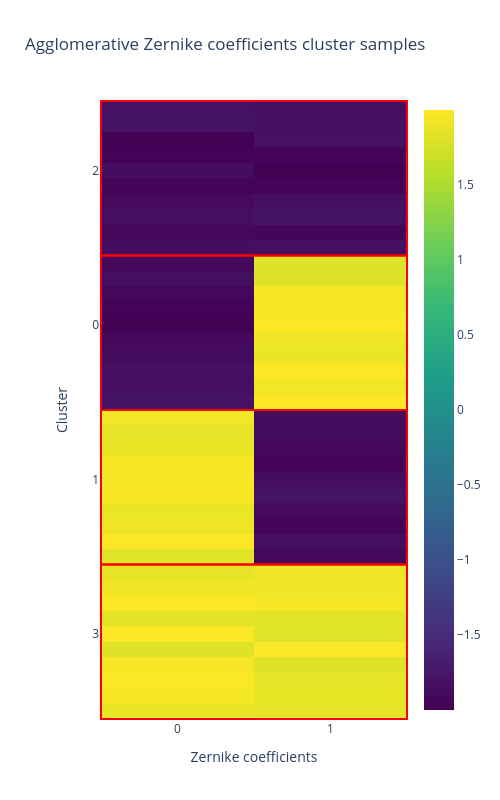
\includegraphics[width=0.4\textwidth]{mdid-zernikecoefficientsAgglomerativegridclusters.png}}
				\caption{Comparison between original clustering and Agglomerative clustering}
			\end{figure*}
		\FloatBarrier
		
		\subsubsection{Summary}
			\begin{figure*}[ht!]
				\centering
				\subfloat[Original cluster densities]{%
					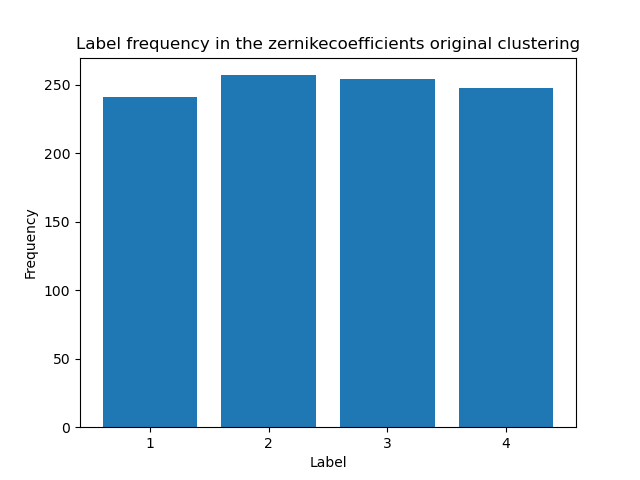
\includegraphics[width=0.18\textwidth]{mdid-zernikecoefficientsoriginaldensity.png}}
				\hspace{\fill}
				\subfloat[K-means cluster densities]{%
					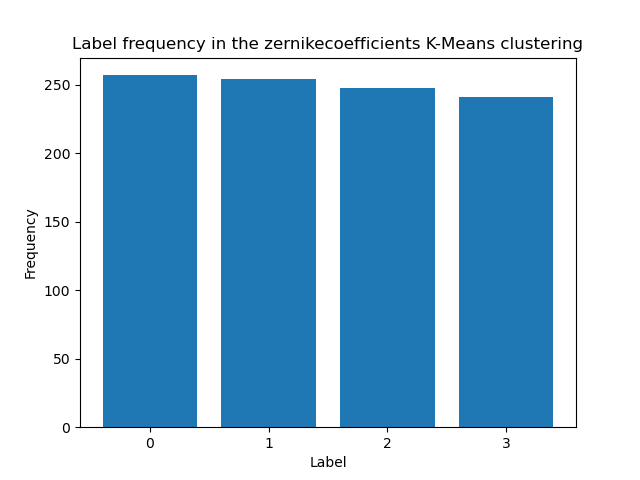
\includegraphics[width=0.18\textwidth]{mdid-zernikecoefficientsK-Meansdensity.png}}
				\hspace{\fill}
				\subfloat[DBSCAN cluster densities]{%
					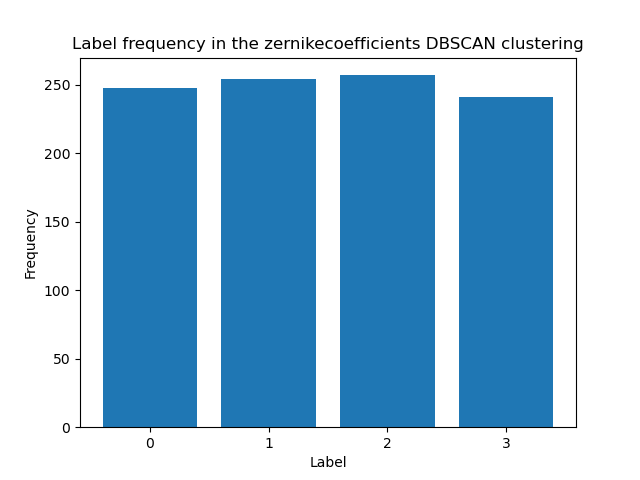
\includegraphics[width=0.18\textwidth]{mdid-zernikecoefficientsDBSCANdensity.png}}
				\hspace{\fill}
				\subfloat[HDBSCAN cluster densities]{%
					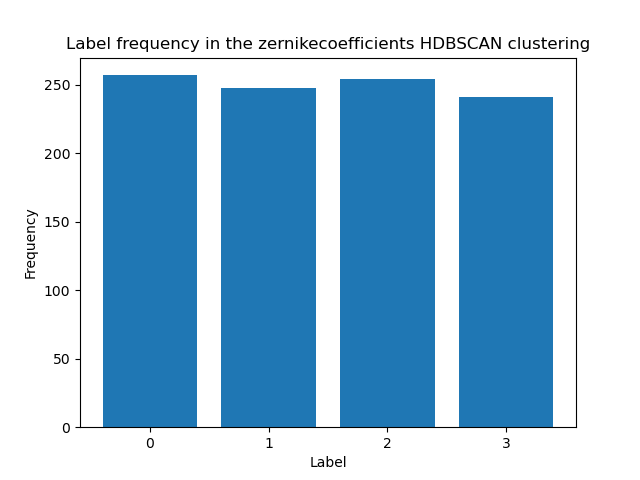
\includegraphics[width=0.18\textwidth]{mdid-zernikecoefficientsHDBSCANdensity.png}}
				\hspace{\fill}
				\subfloat[Agglomerative cluster densities]{%
					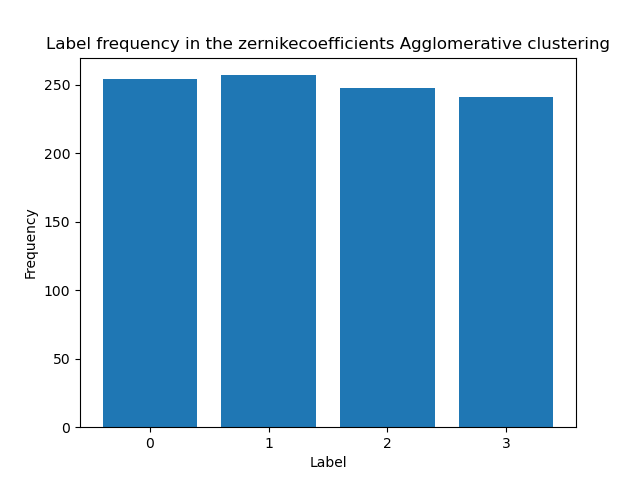
\includegraphics[width=0.18\textwidth]{mdid-zernikecoefficientsAgglomerativedensity.png}}
				\\
				
				\subfloat[Original cluster]{%
					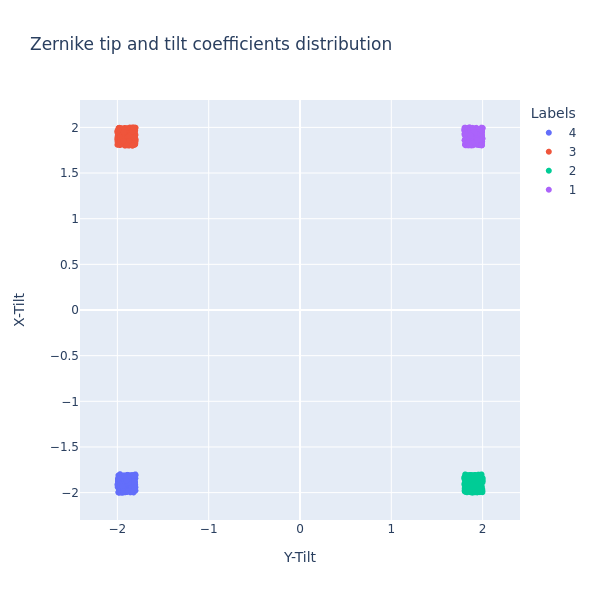
\includegraphics[width=0.18\textwidth]{mdid-originalclusters.png}}
				\hspace{\fill}
				\subfloat[K-means clusters]{%
					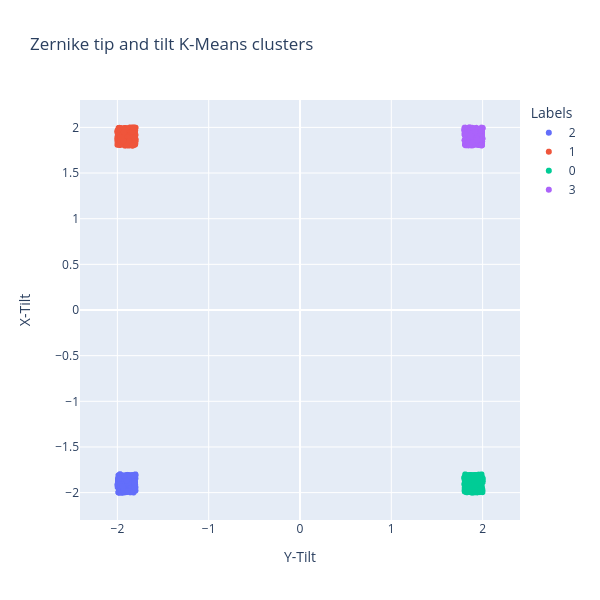
\includegraphics[width=0.18\textwidth]{mdid-zernikecoefficientsK-Meansclusters.png}}
				\hspace{\fill}
				\subfloat[DBSCAN cluster clusters]{%
					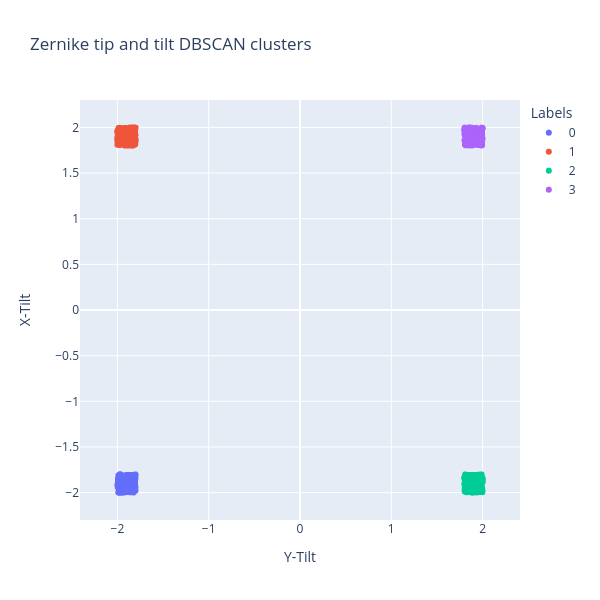
\includegraphics[width=0.18\textwidth]{mdid-zernikecoefficientsDBSCANclusters.png}}
				\hspace{\fill}
				\subfloat[HDBSCAN clusters]{%
					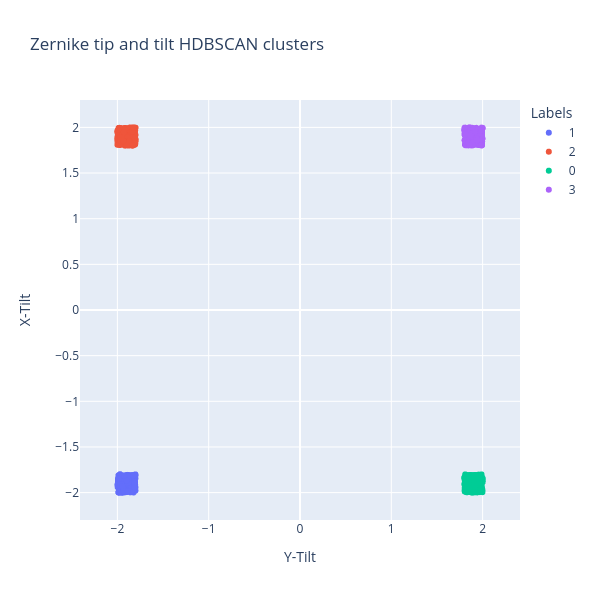
\includegraphics[width=0.18\textwidth]{mdid-zernikecoefficientsHDBSCANclusters.png}}
				\hspace{\fill}
				\subfloat[Agglomerative clusters]{%
					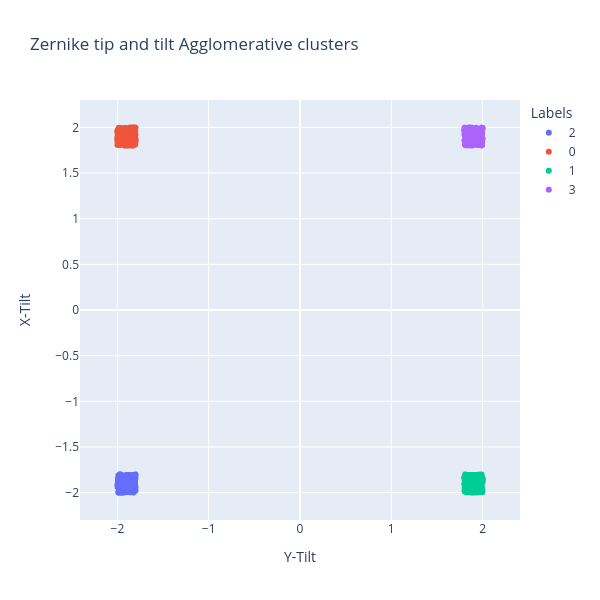
\includegraphics[width=0.18\textwidth]{mdid-zernikecoefficientsAgglomerativeclusters.png}}\\
				
				\subfloat[Original cluster samples]{%
					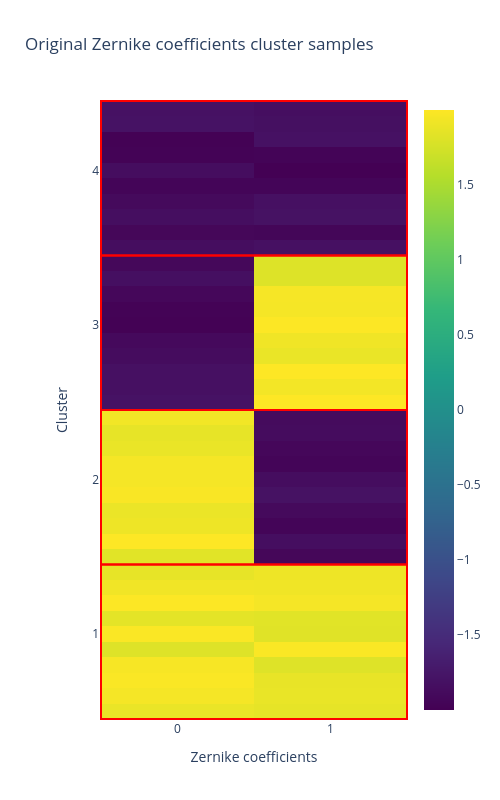
\includegraphics[width=0.18\textwidth]{mdid-zernikecoefficientsoriginalgridclusters.png}}
				\hspace{\fill}
				\subfloat[K-means cluster samples]{%
					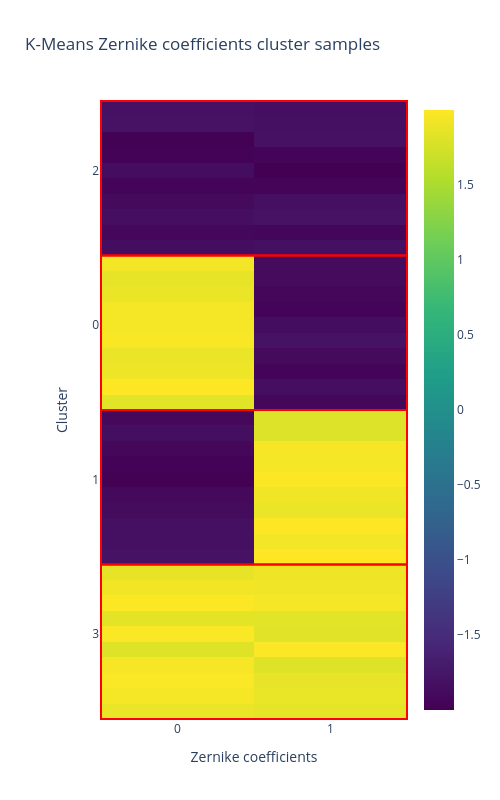
\includegraphics[width=0.18\textwidth]{mdid-zernikecoefficientsK-Meansgridclusters.png}}
				\hspace{\fill}
				\subfloat[DBSCAN cluster samples]{%
					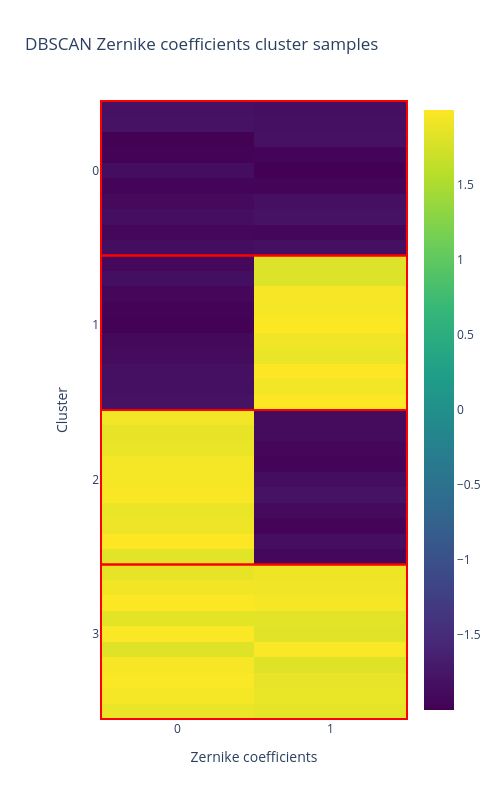
\includegraphics[width=0.18\textwidth]{mdid-zernikecoefficientsDBSCANgridclusters.png}}
				\hspace{\fill}
				\subfloat[HDBSCAN cluster samples]{%
					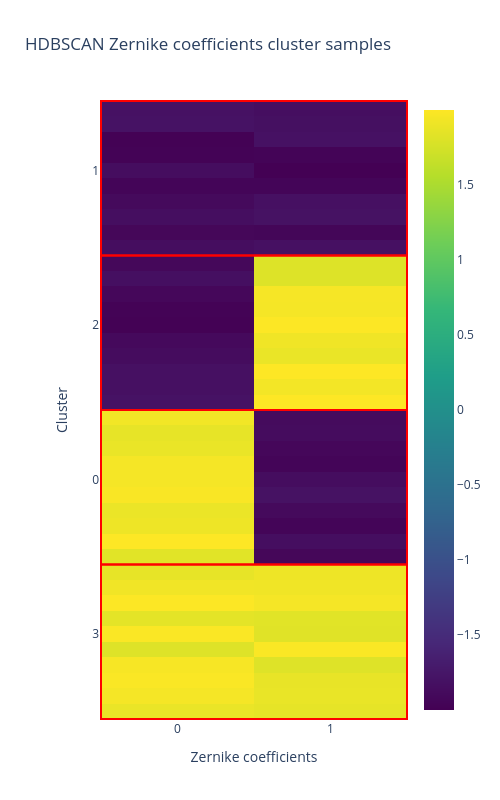
\includegraphics[width=0.18\textwidth]{mdid-zernikecoefficientsHDBSCANgridclusters.png}}
				\hspace{\fill}
				\subfloat[Agglomerative cluster samples]{%
					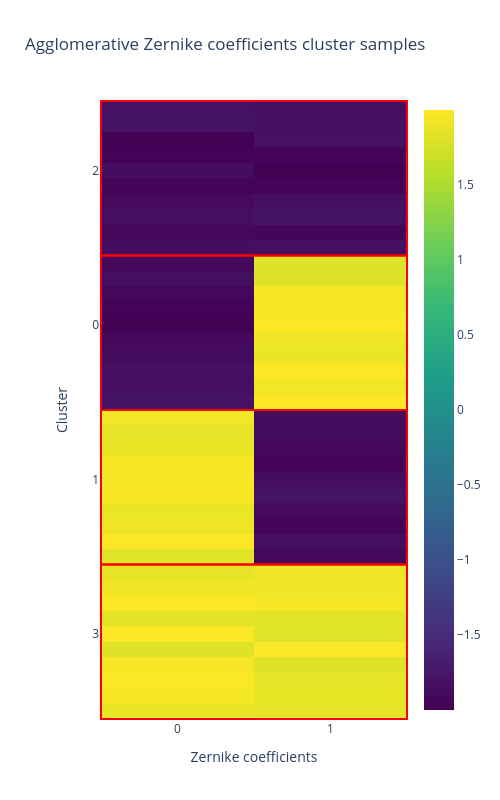
\includegraphics[width=0.18\textwidth]{mdid-zernikecoefficientsAgglomerativegridclusters.png}}
				
				\caption{Comparison between clustering algorithms}
			\end{figure*}
		\FloatBarrier
		
		\begin{table}[h!]
    			\centering
    			\begin{tabular}{|c|c|c|c|c|c|}
        			\hline
        			& \textbf{Original} & \textbf{K-Means} & \textbf{DBSCAN} & \textbf{HDBSCAN} & \textbf{Agglomerative} \\
        			\hline
        			\textbf{Original} & \diagbox{}{} & 1 & 1 & 1 & 1 \\
       			\hline
        			\textbf{K-Means} &  & \diagbox{}{} & 1 & 1 & 1\\
        			\hline
        			\textbf{DBSCAN} &  &  & \diagbox{}{} & 1 & 1\\
        			\hline
        			\textbf{HDBSCAN} &  &  &  & \diagbox{}{} & 1\\
       			\hline
    			\end{tabular}
    			\caption{Normalized Mutual Information between clusters}
		\end{table}